%! app: regular-languages 
%! outcome: Regular expressions, Formal definition of automata, Informal definition of automata

{\bf Review}: Determine whether each statement below about regular expressions
over the alphabet $\{a,b,c\}$ is true or false:
   
True or False: \qquad 
   $a  \in L(~(a \cup b )~\cup c)$

True or False: \qquad 
   $ab  \in L(~ (a \cup b)^*  ~)$
   
True or False: \qquad    
   $ba \in L( ~ a^* b^* ~)$
   
True or False: \qquad 
   $\varepsilon  \in L(a \cup b \cup c)$
   
True or False: \qquad 
   $\varepsilon  \in L(~ (a \cup b)^*  ~)$

True or False: \qquad 
   $\varepsilon \in L( ~ a^* b^* ~)$


{\bf From the pre-class reading, pages 34-36}:
A deterministic finite automaton (DFA) is specified by  $M = (Q, \Sigma, \delta, q_0, F)$.
This $5$-tuple is called the {\bf formal definition} of the DFA. The DFA can also 
be represented by its state diagram: with nodes for the state, labelled edges specifying the 
transition function, and decorations on nodes denoting the start and accept states.

\begin{quote}
Finite set of states $Q$ can be labelled by any collection of distinct names. Often
we use default state labels $q0, q1, \ldots$ 
\end{quote}

\begin{quote}  
The alphabet $\Sigma$ determines the possible inputs to the automaton. 
Each input to the automaton is a string over  $\Sigma$, and the automaton ``processes'' the input
one symbol (or character) at a time.
\end{quote}

\begin{quote}
The transition function $\delta$ gives the next state of the DFA based on the current state of 
the machine and on the next input symbol.
\end{quote}

\begin{quote}
The start state $q_0$ is an element of $Q$.  Each computation of the machine starts at the  start  state.
\end{quote}

\begin{quote}
The accept (final) states $F$ form a subset of the states of the DFA, $F \subseteq  Q$. 
These states are used to flag if the machine accepts or rejects an input string.
\end{quote}


\begin{quote}
The computation of a machine on an input string is a sequence of states
in the machine,  starting with the start state, determined by transitions 
of the machine as it reads successive input symbols.
\end{quote}

\begin{quote}
The DFA $M$ accepts the given input string exactly when the computation of $M$ on the input string
ends in an accept state. $M$ rejects the given input string exactly when the computation of 
$M$ on the input string ends in a nonaccept state, that is, a state that is not in $F$.
\end{quote}

\begin{quote} 
The language of $M$, $L(M)$, is defined as the set of  all strings that are each accepted 
by the machine $M$. Each string that is rejected by $M$ is not in $L(M)$.
The language of $M$ is also called the language recognized by $M$.
\end{quote}   
   
What is {\bf finite} about all deterministic finite automata? (Select all that apply)
\begin{itemize}
   \item[$\square$] The size of the machine (number of states, number of arrows)
   \item[$\square$] The number of strings that are accepted by the machine
   \item[$\square$] The length of each computation of the machine
\end{itemize}
  
\begin{figure}[h]
   \centering
   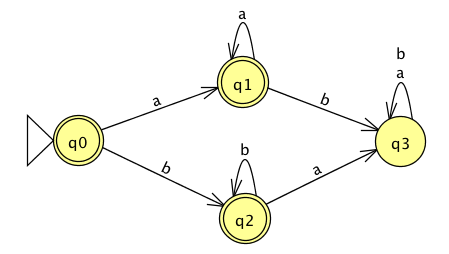
\includegraphics[width=3in]{../../resources/machines/Lect2DFA1.png} 
\end{figure}
   
The formal definition of this DFA is
   
\vspace{100pt}
   

Classify each string $a, aa, ab, ba, bb, \varepsilon$ as accepted by the DFA or rejected by the DFA.  

{\it Why are these the only two options?}

\vspace{200pt}


The language recognized by this DFA is
  
\vspace{100pt}
   

\begin{figure}[h]
  \centering
  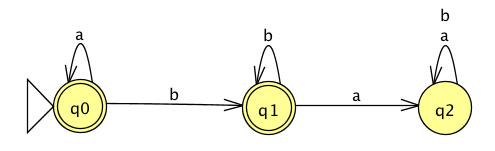
\includegraphics[width=3in]{../../resources/machines/Lect2DFA2.png} 
\end{figure}
   

The language recognized by this DFA is
  
\vspace{100pt}

\begin{figure}[h]
    \centering
    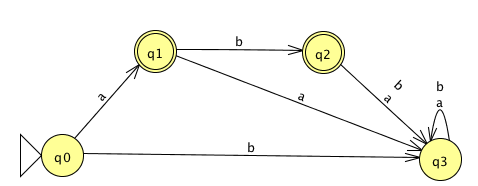
\includegraphics[width=3in]{../../resources/machines/Lect2DFA3.png} 
\end{figure}

The language recognized by this DFA is
  
\vspace{100pt}
